\documentclass{article}
\usepackage[utf8]{inputenc}
\usepackage{amsmath}
\usepackage{graphicx}

\title{CS 377P Assignment 2}
\author{Joseph Bess, Krishna Ramdeep}
\date{February 2018}

\begin{document}

\maketitle

\section{Iterative Solution of Linear Systems}
\par
a) The recurrence relation for the linear system \[3x-4y=-1\] \[x+2y=3\] can be expressed as follows: \[x_{i+1} = x_i-\frac{1}{3}(3x_i-4y_i+1)\] \[y_{i+1} = y_i-\frac{1}{2}(x_i+2y_i-3)\]\\
Expressed in terms of matrices and vectors, the recurrence becomes:\\ \[\begin{pmatrix}x_{i+1}\\y_{i+1}\end{pmatrix}=\begin{pmatrix}x_i\\y_i\end{pmatrix}-\begin{pmatrix}\frac{1}{3} & 0\\0 & \frac{1}{2}\end{pmatrix}\begin{pmatrix}3x_i-4y_i+1\\x_i+2y_i-3\end{pmatrix}\]
Where $\begin{pmatrix}\frac{1}{3} & 0\\0 & \frac{1}{2}\end{pmatrix}$ is the inverse of the diagonal coefficient matrix.
\newpage
b) The plot:
\begin{center}
    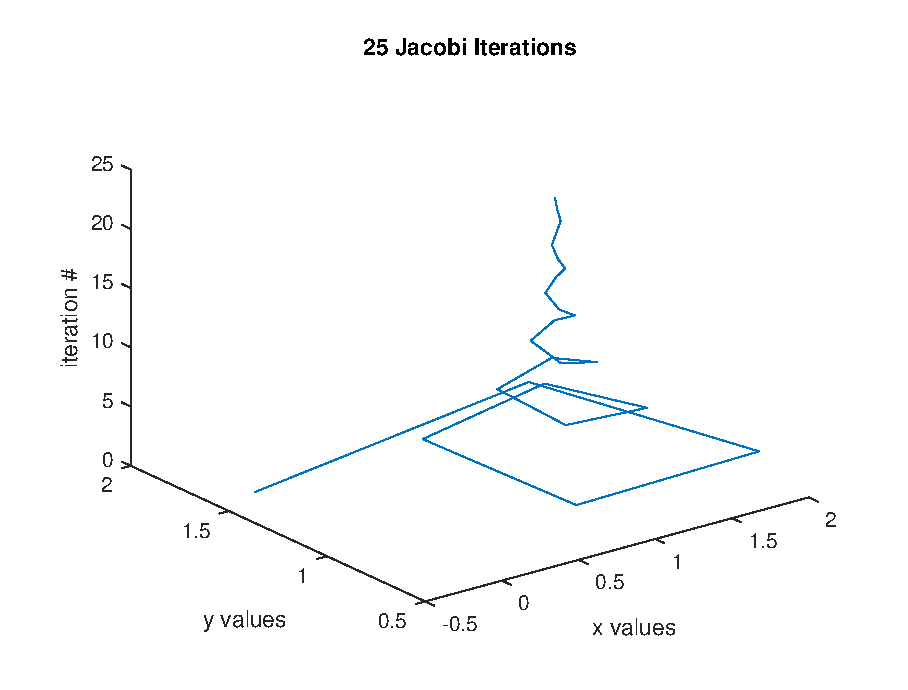
\includegraphics[scale = 0.8]{jacobi25.eps}
\end{center}
This plot looks as one would expect, as we can see that as the number of iterations increases (in the positive z-direction), the $x, y$ values converge towards the actual solutions of the linear system $(x = 1, y = 1)$.
\newpage
c) The recurrence relation is: \[x_{i+1} = x_i-\frac{1}{3}(3x_i-4y_i+1)\] \[y_{i+1} = y_i-\frac{1}{2}(x_{i+1}+2y_i-3)\]
The plot:
\begin{center}
    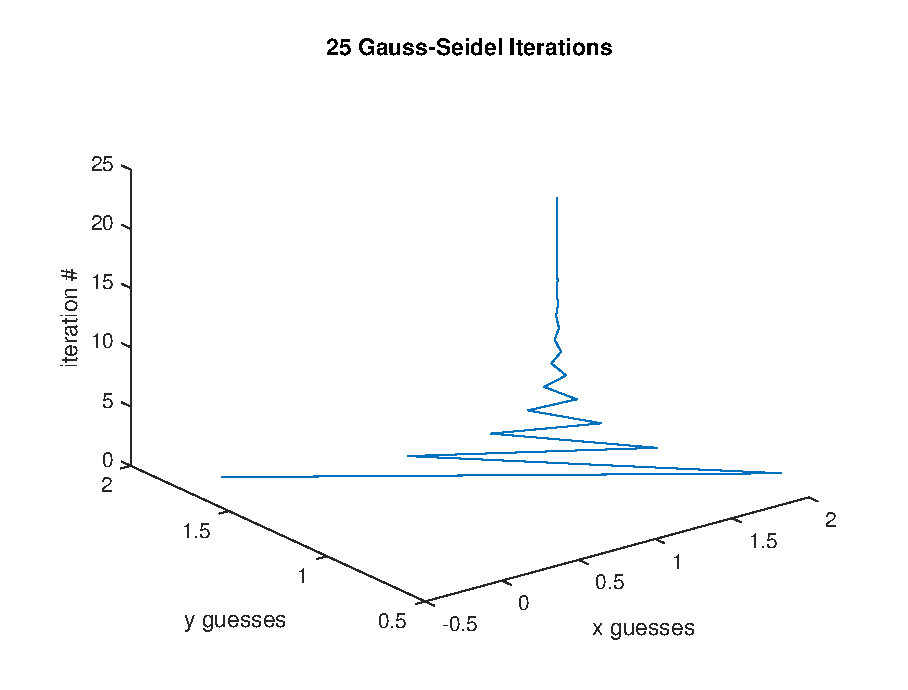
\includegraphics[scale = 0.8]{gs25.eps}
\end{center}
This plot looks as one would expect, but notice that Gauss-Seidel converges much faster for this system.
\newpage
\section{Ordinary Differential Equations}
\par
a) The recurrence relation for estimating the forward step: \[y((i+1)*h)=y(ih)(h*sin(x)+1)\]
The graph is:
\begin{center}
    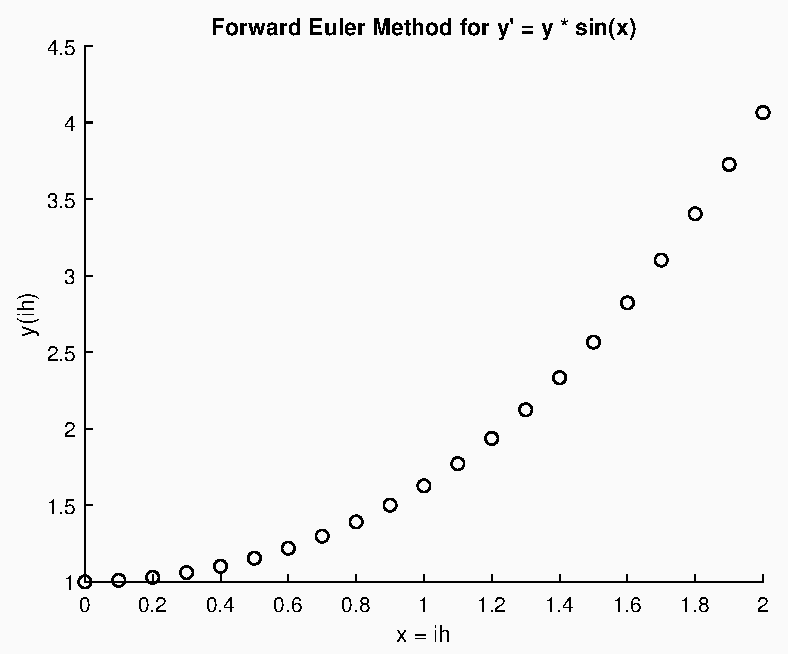
\includegraphics[scale = 0.8]{feuler2a.eps}
\end{center}
\newpage
b) It makes sense that $y_c(h)=1$ since $y_c(0)=1$. Since the derivative at 0 is 0, there is no change. The recurrence relation is: \[y((i+1)*h)=2hy(ih)sin(x)+y((i-1)*h)\]
The graph is:
\begin{center}
    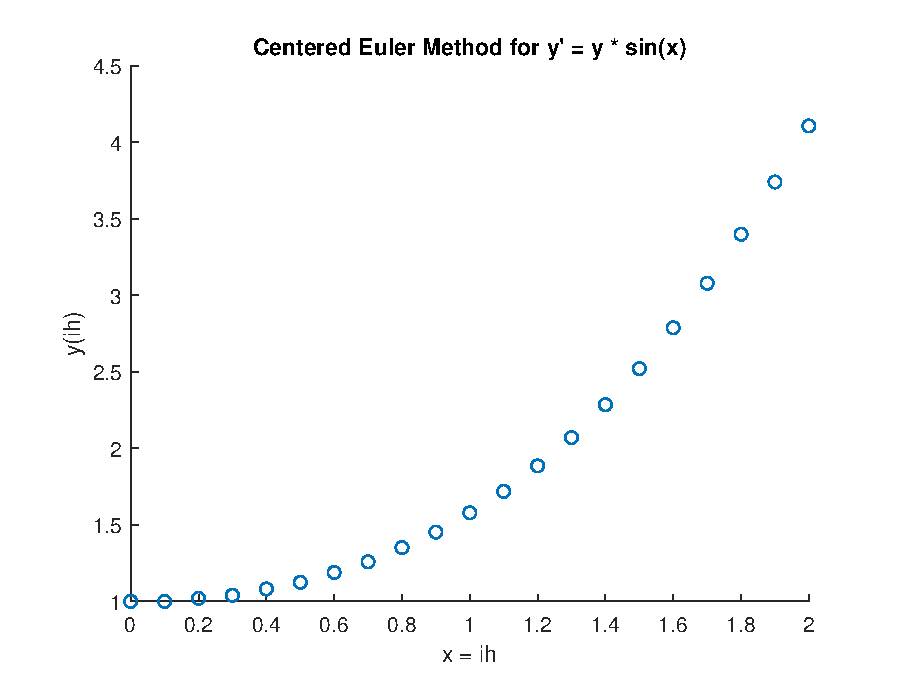
\includegraphics[scale = 0.8]{center2b.eps}
\end{center}
\newpage
\section{Partial Differential Equations}
\par
a) The stencil looks like this:
\begin{center}
    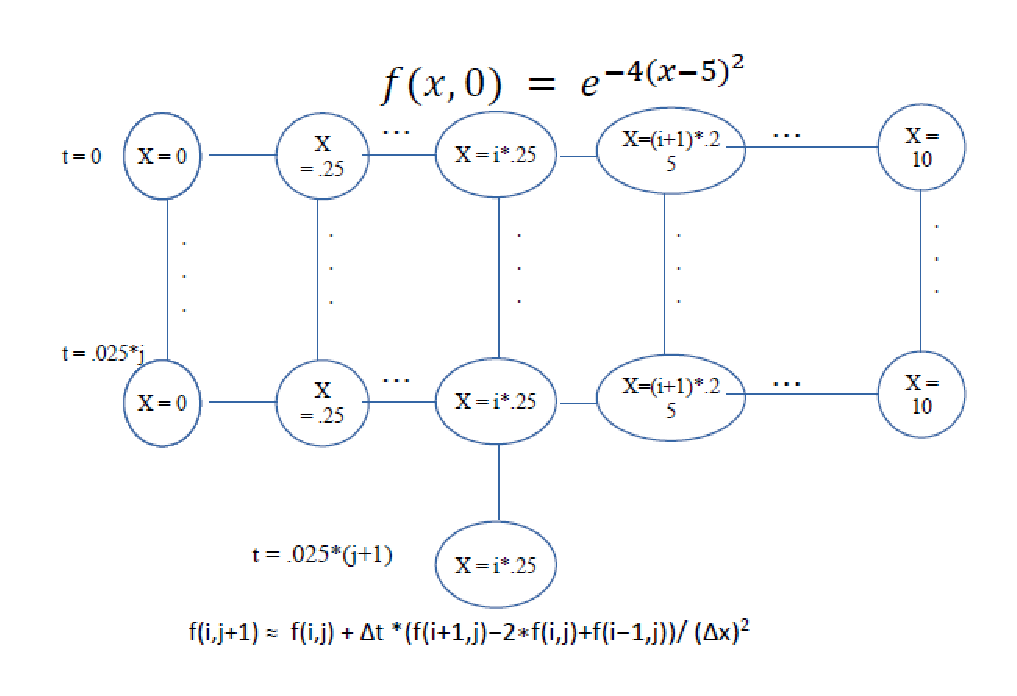
\includegraphics[scale = 0.8]{stencil.eps}
\end{center}
b) The recurrence relation is: \[\hat{f}(i,j+1)=\hat{f}(i,j)+0.4*(\hat{f}(i+1,j)-2\hat{f}(i,j)+\hat{f}(i-1,j))\] The 0.4 is just a constant obtained from the term $\frac{\Delta t}{(\Delta x)^2}$.
The graph is:
\begin{center}
    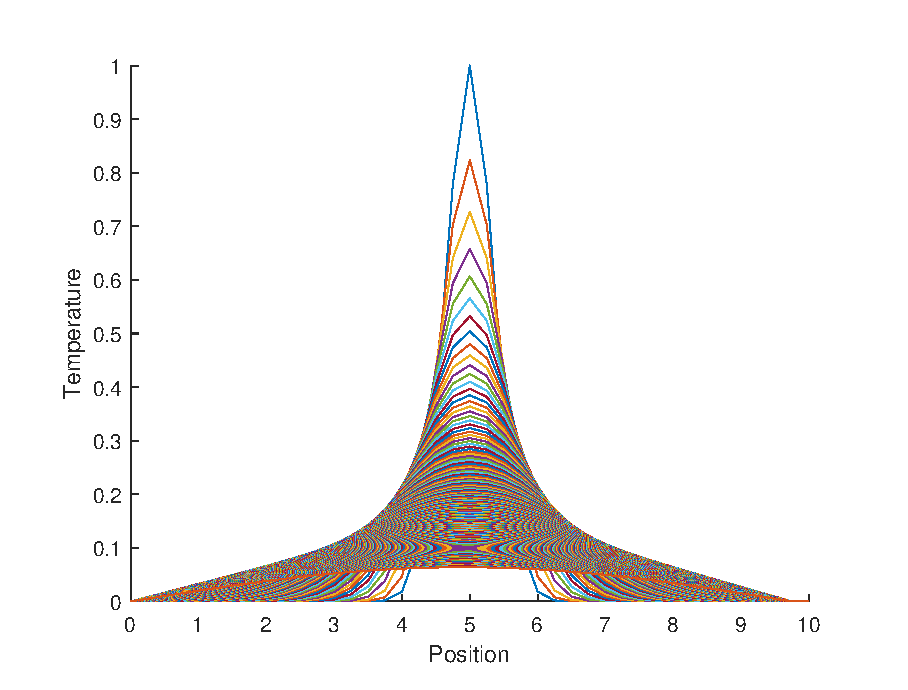
\includegraphics[scale = 0.8]{firsttimestep.eps}
\end{center}
This does jive with our intuition.\\
c) This is the new graph:
\begin{center}
    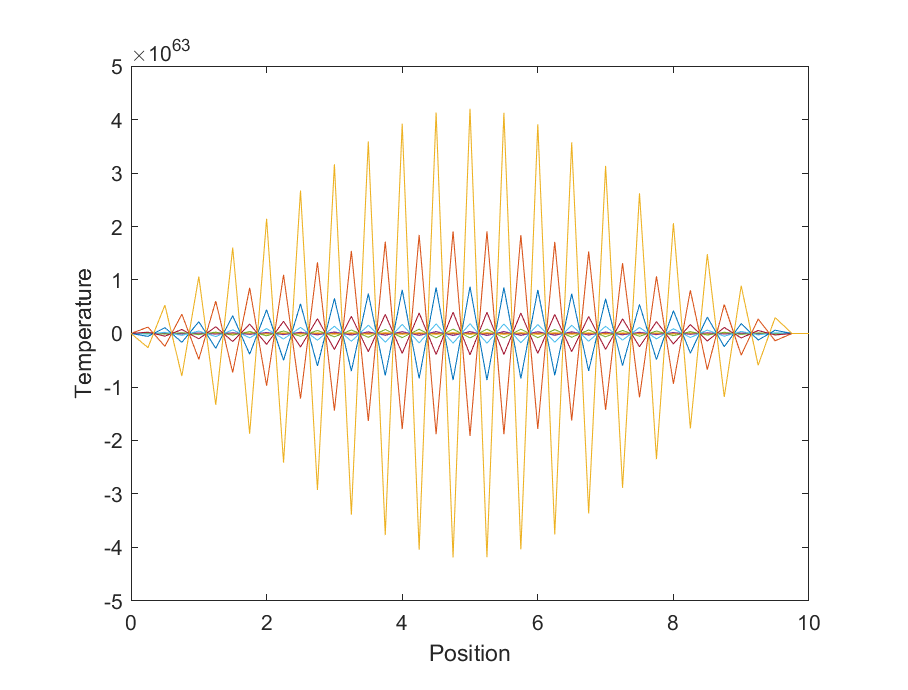
\includegraphics[scale = 0.8]{secondtimestep.eps}
\end{center}
Our best guess is that since we are using forward-euler to approximate $\frac{\delta f}{\delta t}$, we are seeing oscillation in the graph.
\end{document}
